%*************************************************************
% Master Thesis                                             *
% Ing. Minerva Gabriela Vargas Gleason                       *
%  IAI Institute of Artificial Intelligence                   *
% Universität Bremen                                         *
%                                                            *
% pdfLaTex                                                   *
% Editor: TeXnicCenter                                       *
%*************************************************************


\chapter{\textbf{Introduction}}

Motion planning and trajectory generation is a central part of robotics. Being able to parametrize the movements a robot execute is crucial for the flexibility of the system and an important step in the robot-human interaction field.

The number and applications of robots in our society is growing day by day, we can find them in production lines, at hospitals, as guides in museums and even at home, just to mention some examples. The capabilities and autonomy required by each robot widely varies depending on its application. One often addressed problem in robotics is object manipulation.

The aim of this work is to develop the \textit{motion generation component} of a \textit{grasping system} based on a whole-body robot motion controller. The system must be able to obtain a trajectory that a robot has to execute in order to grasp a specified object. This implies the system detects the object and generates a trajectory for a mechanical system with multiple degrees of freedom (DOFs) that successfully reaches a position and orientation under given initial conditions.

The developed system will be implemented and tested on the Boxy robot (figure \ref{fig:boxy}), a dual-armed robot from the Institute for Artificial Intelligence\footnote{http://ai.uni-bremen.de/research/robots/boxy} (IAI). The trajectory generation system currently used by Boxy is Giskard (section \ref{subsec:giskard}), an optimization-based controller developed at the IAI. 

The main contributions of this work are implementing a collision detection system and limiting the acceleration of the robot while planning, as well as the ability of deciding on its own how an object should be grasped.

\section{Motivation}
% What is the problem?
In the 1960's the robots were introduced in the industry. They were mainly used at the automotive industry for pick and place tasks  \citep{history}. Robots replaced humans in monotonous, hard and dangerous tasks. 

Most industrial robots used in assembly lines have no sensors that gives them information about their environment, they work by moving from one predefined position to the next one, executing controlled trajectories. Robots working without external information have to be kept in a controlled environment, where the position of all objects is known beforehand and they only have to execute a repetitive task.

Nowadays, service robots are envisioned to work in a wide range of situations where they dynamically interact with their environment, where the position of objects and obstacles is not known beforehand and can continuously change. Working under these conditions requires some degree of autonomy from the system.

One of the central questions this thesis address is how can one parametrize the trajectory generation for a robot in an object grasping scenario, so that the robot is able to decide how it's movement should be under given conditions and successfully execute a grasping movement.

An important point of this work is to understand the behavior of an optimization-based and constraint-based robotic motion controller, to find out which constraints are relevant for the trajectory generation and how each one of these constraints affects the controller's output.

% Why is it a hard problem?
Object grasping and manipulation  constitutes a big challenge in the robotics field. In order to successfully grasp an object, the robot must:
\begin{itemize}
	\item Identify the object and its position with respect to the robot. This is done by a perception system which analyzes the information provided from sensors, normally cameras.
	\item Decide how to grasp the object. Usually, an object can be grasped in several ways. Taking a cup as example, it can be grabbed from the handle, from the cup body or from the top edge (figure \ref{fig:obj_grasp_pose}). The system should be able to decide which one of this \textbf{grasping poses} is better depending on the situation.
	\item Generate trajectories that move the end effector (EEF) from its current location to the selected grasping pose. This includes trajectory generation and motion control.
	\item Evaluate if the obtained trajectories will generate a collision with the robot itself or the environment. Discard the trajectories where collisions were detected.
	\item Send the best trajectory to a PI controller that will send the corresponding commands to the robot to execute it.
\end{itemize}

Being able to grasp an object is an essential ability in robot manipulation. Having a system that autonomously locates and grasp an object using \textit{On-line Trajectory Generation (OTG)} gives great flexibility to the robot. OTG grants the capability of modifying the trajectory during execution, it implies recalculating the trajectory on every control cycle . By doing this, the system is able to react instantaneously to unexpected events, such as a change in the goal position.

\begin{figure}[H]
	\centering
	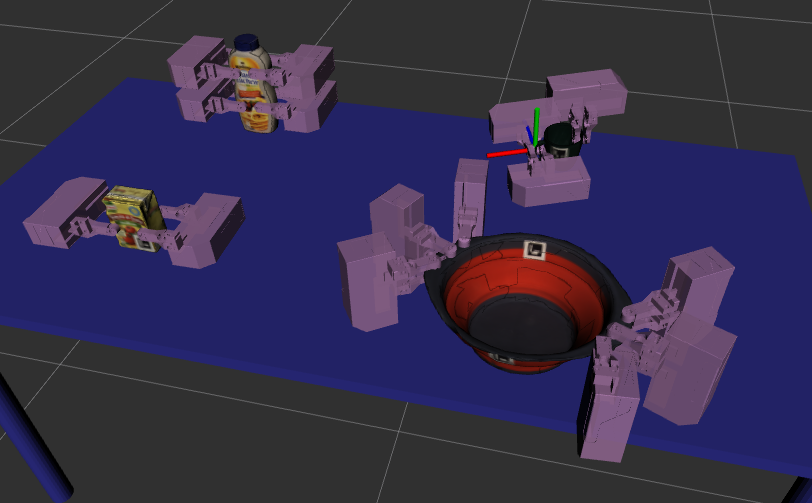
\includegraphics[width=0.55\linewidth, angle=0]{multiple_objects.png}
	\vspace{-10pt}
	\caption{Example of objects with predefined grasping poses}
	\vspace{-15pt}
	\label{fig:obj_grasp_pose}
\end{figure}

The proposed solution to this grasping problem includes generating a data base of objects with predefined grasping poses (GP) (figure \ref{fig:obj_grasp_pose}) and a perception system that detects the stored objects and shows the possible GP and it's position with respect to the robot.

The robot will have to decide which GP is better for grasping a specified object given a initial configuration. Then, an optimization controller (section \ref{sec:motion_controller}) will generate several possible trajectories, evaluate them and send the best one to the Boxy robot (figure \ref{fig:boxy}).

\begin{figure}[H]
	\centering
	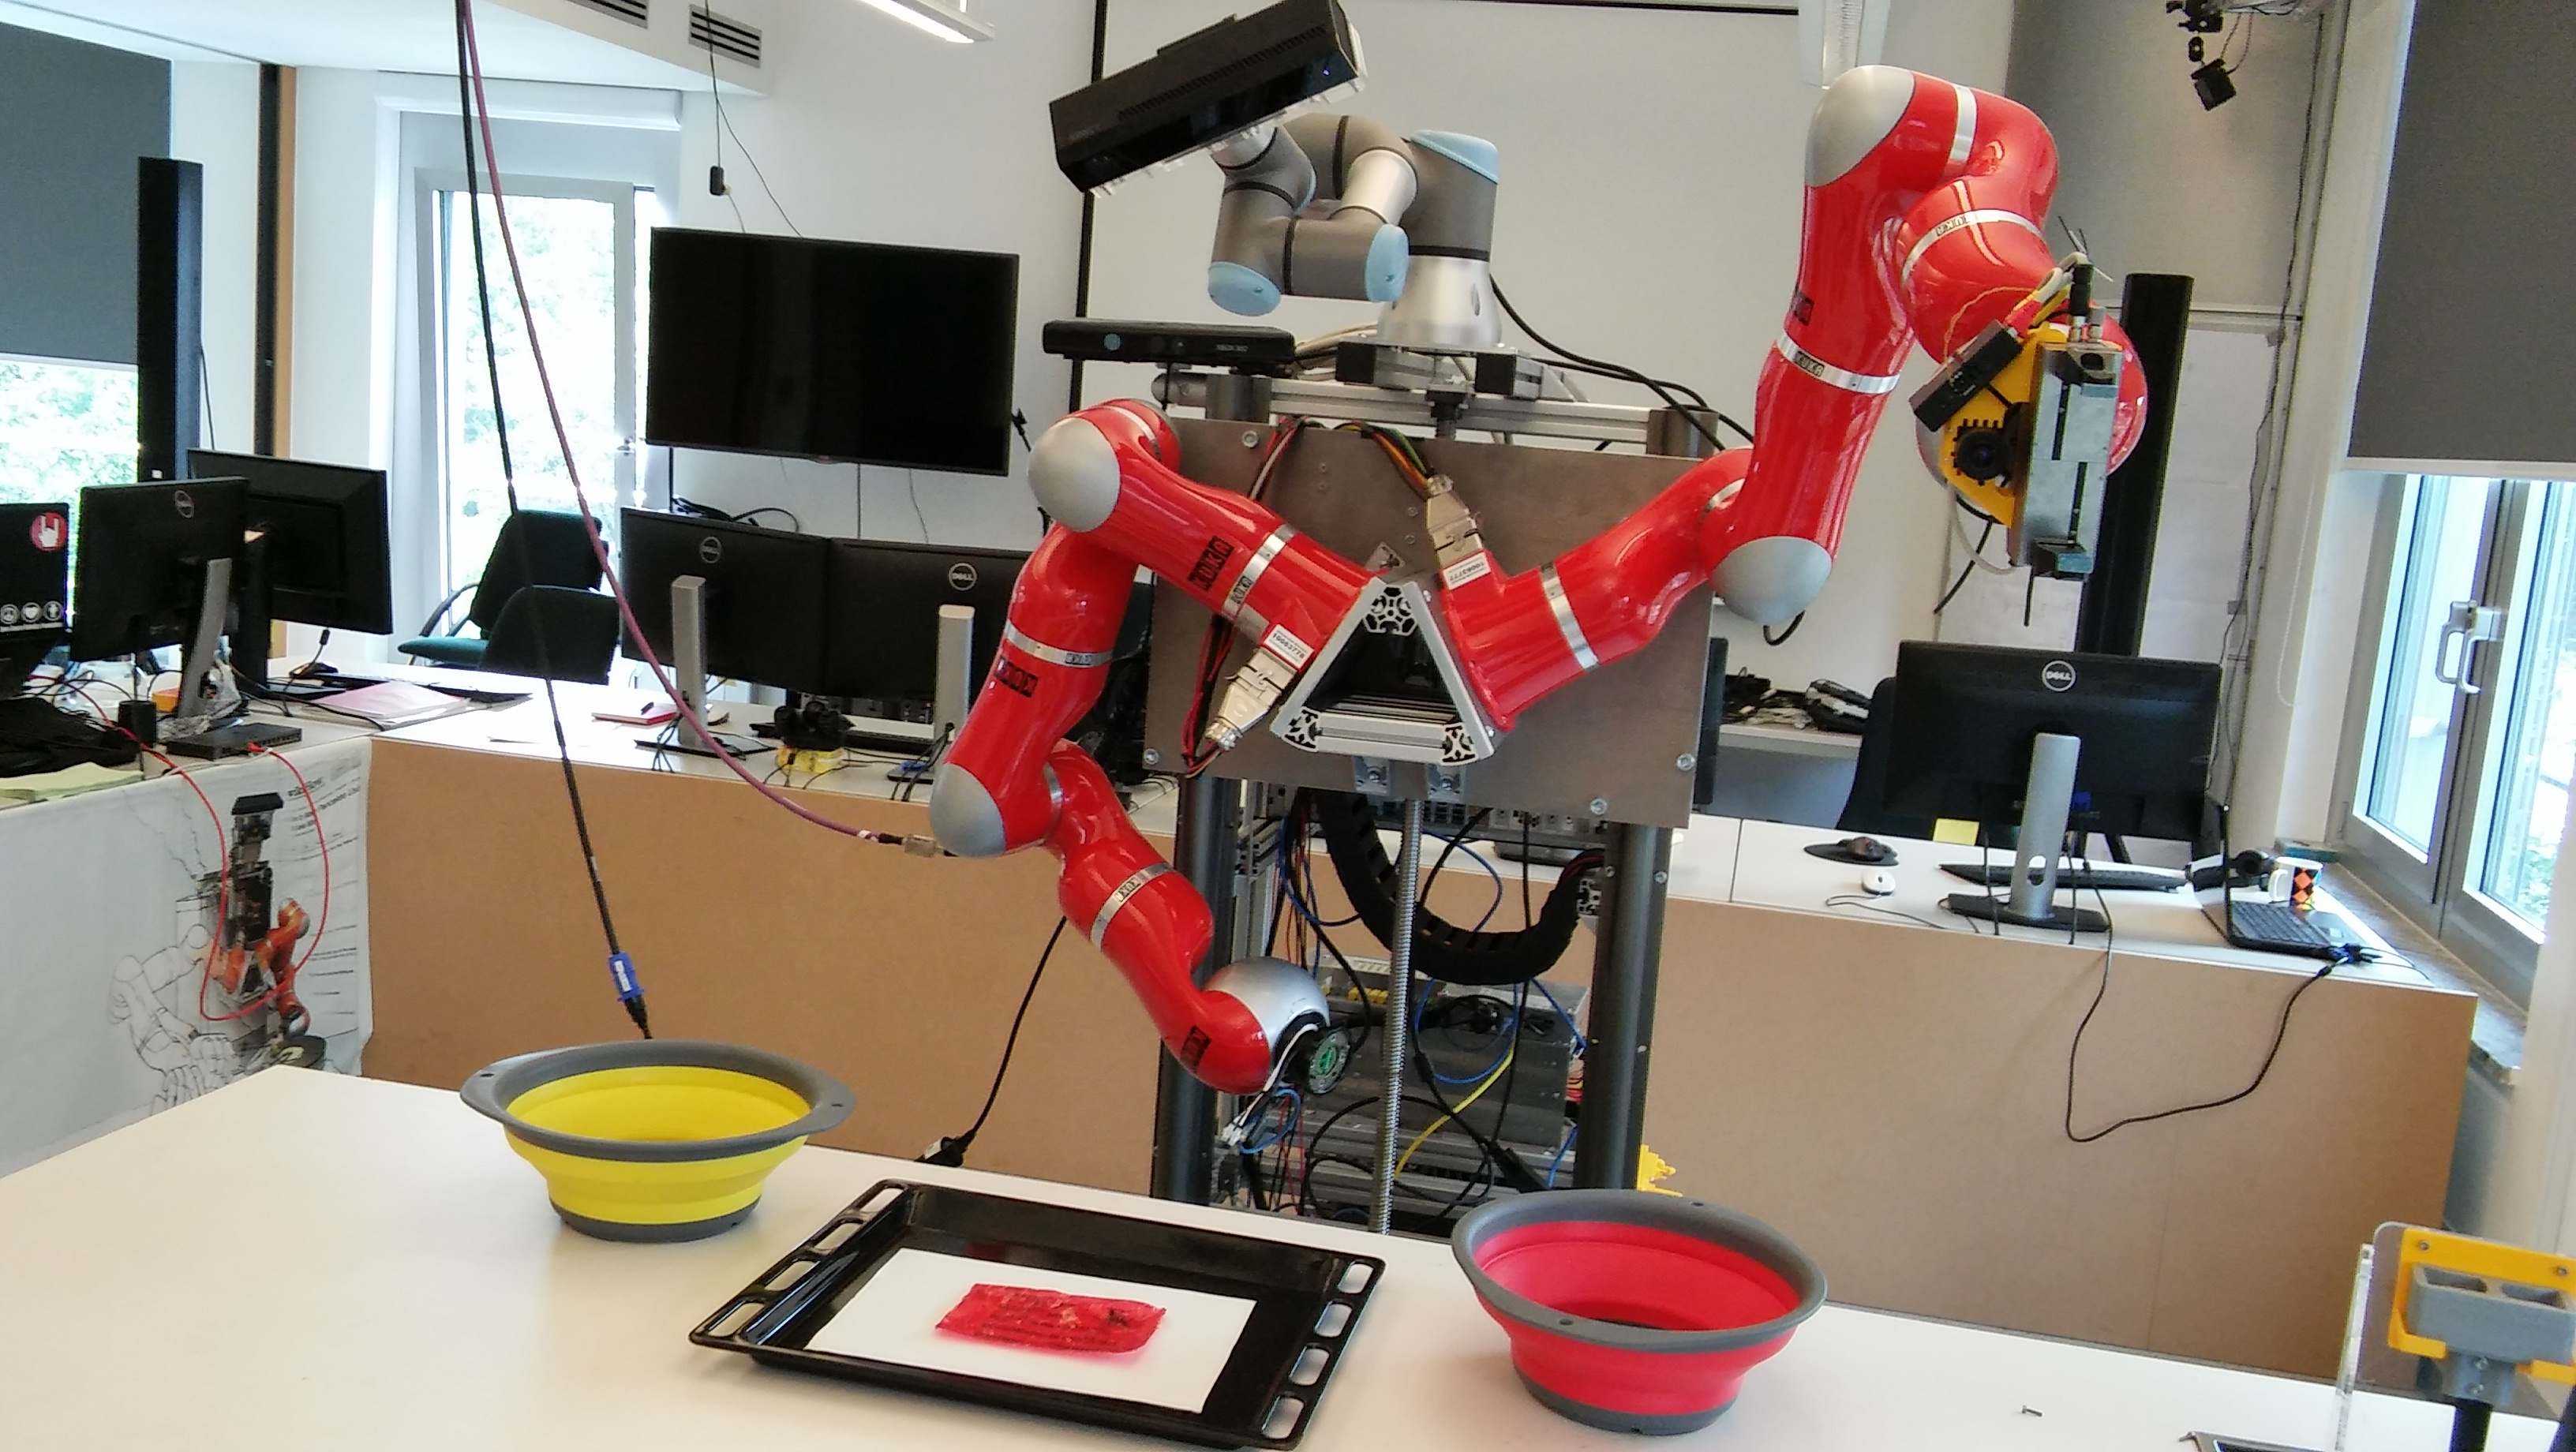
\includegraphics[width=0.55\linewidth, angle=0]{boxy/Boxy3.jpg}
	\vspace{-10pt}
	\caption{The Boxy robot}
	\vspace{-15pt}
	\label{fig:boxy}
\end{figure}

As result, it is expected a system with a parametrized motion controller that generates a smooth trajectory for Boxy by limiting the velocity and acceleration of each joint. The system should be able to decide which grasping pose (GP) of a selected object can be better grasped given the current system conditions.

% Why is this an interesting problem? If solved, what is then possible?
% What is your approach to solving this problem?

\section{Contributions}
% Data, software, algorithms, designs, etc... made by me. If the problem was solved, how was that done?

The main contribution of this work was the development of a projection system for trajectory planning (section \ref{sec:sys_description}). This system uses a naive kinematic simulator (section \ref{sub:naive}) of the robot to generate several possible trajectories. Each one of the obtained trajectories is evaluated and scored and one is selected to be executed by the real robot. Some of the evaluation criteria are trajectory smoothness and length, manipulability of the robot after the goal position is reached and collisions during the trajectory simulation.

The collision detection was developed using Moveit! Planning scene\footnote{http://moveit.ros.org/} (section \ref{subsec:moveit}). The system is not able to consider collision avoidance while generating a trajectory, but the collision detection system discards all trajectories that would generate a collision with the robot itself or with the environment (section \ref{sec:collision}).

During the development of this work, an object database was created(section \ref{sec:db}) with 3D models of several objects and predefined grasping poses for each object. The object models were created using a 3D scanner. The gripper and furniture models were done in a CAD program.

In order to detect the objects located in front of the robot, I developed a perception system that uses fiducial markers as side product (section \ref{sec:perception}).

The robot moves by receiving a sequence of velocity commands for the joints, so it is not possible to send a trajectory at once, it has to be sent step by step. A simple PI controller was created to send the obtained trajectory to the robot (section \ref{sec:pi_controller}).


\section{Structure of the thesis}

The first chapter explains the aim of this work and the motivation behind it, as well as the outcomes of it. The second chapter explains the theory behind the algorithms of this thesis and some useful concepts. It starts by describing some basic concepts for trajectory planning in robotics, such as kinematic models and collision environment. Afterwards it explains some motion planning algorithms, including the one used in this work. In the end, it gives a short description of the  software used by the system.

Chapter three depicts all the elements of the system created in this work. First, it shows the system architecture and starts describing them. At first, the perception system is explained, afterwards comes the structure of the database where the object's models and descriptions are stored. The third section explains the motion controller, the main component of this work. Then it gives a brief explanation of the trajectory evaluation and collision checking. Afterward describes the PI controller used to send the trajectories to the Boxy robot.

The fourth chapter displays the results of this works and describes the evaluation of the generated trajectories. It starts by describing the two types of experiments made: simulated and on the real robot,and the environment for each of them. Thereafter, it describes the behavior of the controller during one of the simulated trajectories. Then it shows tables of the generated trajectories, where the evaluation is shown. In the end, the results of the trajectories executed on the real robot are shown.

The fifth and last chapter discuses the results shown in chapter four. It also provides a short summary about the contributions of this work and proposes further improvements. The repercussions and applications of this system are also stated.

For the ones interested in using this work, the appendix provides links to the Github repositories with all the code generated and a short explanation on how to execute it.
